\chapter{Memory operations}



\section{Vivado project}
The Vivado block scheme of the project is shown in Figure \ref{fig:fifo}. 
\begin{figure}[h!t!]
	\centering
	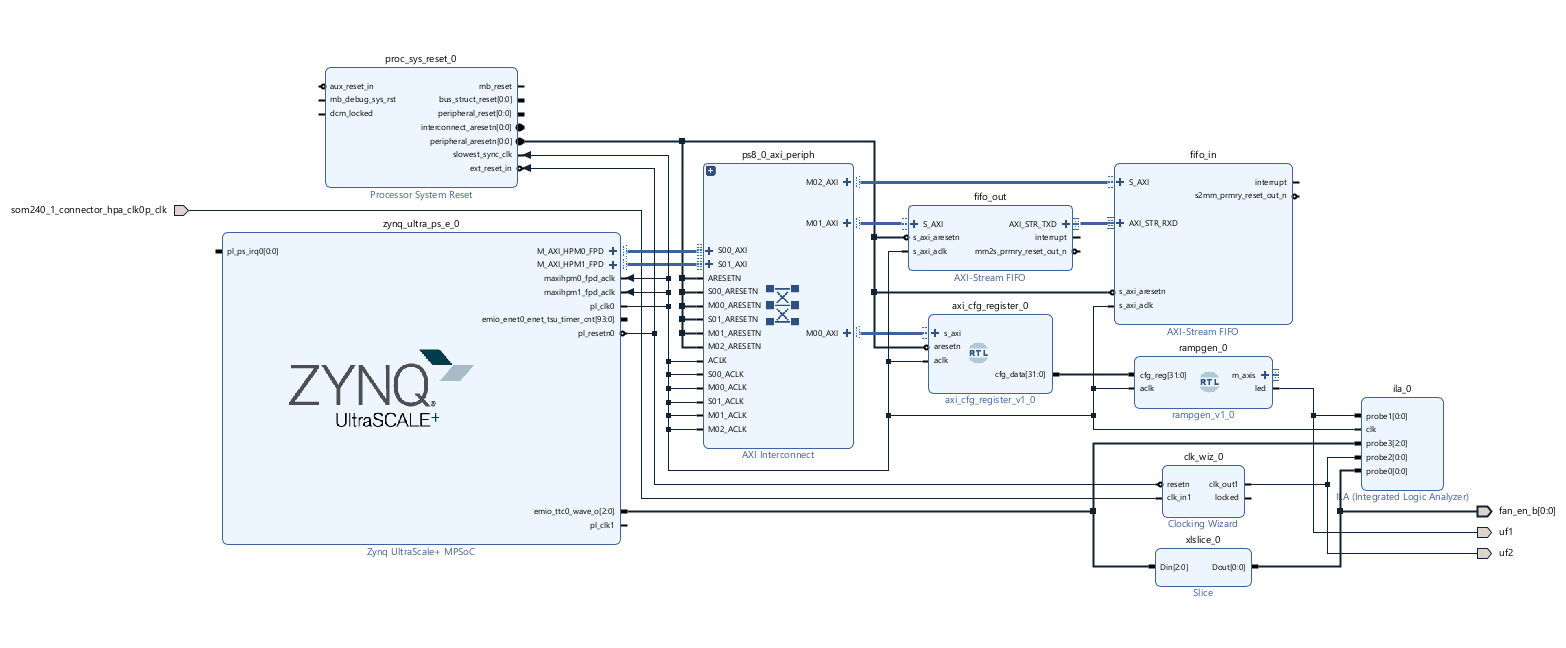
\includegraphics[width=1\textwidth]{images/fifo}
	\caption{Block scheme of the memory operation design project.}
	\label{fig:fifo}
\end{figure}
It is easy to notice that this implementation is more complex than the previous one. In addition to the previously used IP blocks, a few more have been added to enhance functionality. These additional components play a crucial role in enabling efficient data exchange and communication between the Processing System (PS) and Programmable Logic (PL), making the design more sophisticated and capable.

\subsection{Block description}
\paragraph{AXI Interconnect \& Processor System Reset}
These two blocks are automatically imported when the automatic interconnection process is initiated. As a result, there is no need to manually define any code for their integration, as they are handled by the system's design automation tools. The former block facilitates communication between the PS and PL by managing data transfers over the Advanced eXtensible Interface (AXI) protocol. It connects multiple AXI peripherals and ensures efficient data routing. The second block handles the reset signals for the entire system, ensuring that the processor and connected peripherals start in a known, stable state during initialization or after a reset event.

\paragraph{rampgen\_v1.0}
This building block serve to generate the test signal to be written/read by/in the FIFO memories. However, in the current implementation, such block is not used and the data generation is handled directly via software. However, its code is shown below.
\vspace{0.1cm}
\begin{lstlisting}[language=VHDL]
library IEEE;
use ieee.std_logic_1164.all;
use ieee.numeric_std.all;
use ieee.std_logic_misc.all;

entity rampgen is
	Port ( 
	aclk : in STD_LOGIC;
	cfg_reg : in STD_LOGIC_VECTOR (31 downto 0);
	m_axis_tdata        : out std_logic_vector(31 downto 0);
	m_axis_tvalid       : out std_logic;
	m_axis_tready       : in  std_logic;
	m_axis_tlast        : out std_logic;
	led : out STD_LOGIC);
end rampgen;

architecture implementation of rampgen is
	signal prev_reg: STD_LOGIC_VECTOR (31 downto 0);
	signal led_out: STD_LOGIC := '0';
begin
	led <= led_out;
	handle_ramp: process(aclk)
		variable out_count : integer;
	begin
		if rising_edge(aclk)  
		then
			if (prev_reg = "00000000000000000000000000000000" and not (cfg_reg =  "00000000000000000000000000000000")) 
			then 
				out_count := to_integer(signed(cfg_reg(31 downto 0)));
				led_out <= '1';
			end if;
			if out_count > 0 and m_axis_tready = '1' 
			then
				out_count := out_count - 1;
				m_axis_tdata <= std_logic_vector(to_unsigned(out_count, 32));
				m_axis_tvalid <= '1';
				m_axis_tlast <= '1';
			else
				m_axis_tvalid <= '0';
				m_axis_tlast <= '0';
			end if;
			prev_reg <= cfg_reg;
		end if;
	end process; 
end implementation;
\end{lstlisting}

\paragraph{axi\_cfg\_register}
This register facilitates communication between the user and the device. Although it is not utilized in the current implementation, it was previously used to set the initial value for the ramp generator. Its code is reported below.
\vspace{0.1cm}
\begin{lstlisting}[language=Verilog]
`timescale 1 ns / 1 ps

module axi_cfg_register #
(
	parameter integer CFG_DATA_WIDTH = 1024,
	parameter integer AXI_DATA_WIDTH = 32,
	parameter integer AXI_ADDR_WIDTH = 32
)
(
	// System signals
	input  wire                        aclk,
	input  wire                        aresetn,
	
	// Configuration bits
	output wire [CFG_DATA_WIDTH-1:0]   cfg_data,
	
	// Slave side
	input  wire [AXI_ADDR_WIDTH-1:0]   s_axi_awaddr,  // AXI4-Lite slave: Write address
	input  wire                        s_axi_awvalid, // AXI4-Lite slave: Write address valid
	output wire                        s_axi_awready, // AXI4-Lite slave: Write address ready
	input  wire [AXI_DATA_WIDTH-1:0]   s_axi_wdata,   // AXI4-Lite slave: Write data
	input  wire [AXI_DATA_WIDTH/8-1:0] s_axi_wstrb,   // AXI4-Lite slave: Write strobe
	input  wire                        s_axi_wvalid,  // AXI4-Lite slave: Write data valid
	output wire                        s_axi_wready,  // AXI4-Lite slave: Write data ready
	output wire [1:0]                  s_axi_bresp,   // AXI4-Lite slave: Write response
	output wire                        s_axi_bvalid,  // AXI4-Lite slave: Write response valid
	input  wire                        s_axi_bready,  // AXI4-Lite slave: Write response ready
	input  wire [AXI_ADDR_WIDTH-1:0]   s_axi_araddr,  // AXI4-Lite slave: Read address
	input  wire                        s_axi_arvalid, // AXI4-Lite slave: Read address valid
	output wire                        s_axi_arready, // AXI4-Lite slave: Read address ready
	output wire [AXI_DATA_WIDTH-1:0]   s_axi_rdata,   // AXI4-Lite slave: Read data
	output wire [1:0]                  s_axi_rresp,   // AXI4-Lite slave: Read data response
	output wire                        s_axi_rvalid,  // AXI4-Lite slave: Read data valid
	input  wire                        s_axi_rready   // AXI4-Lite slave: Read data ready
);

function integer clogb2 (input integer value);
	for(clogb2 = 0; value > 0; clogb2 = clogb2 + 1) value = value >> 1;
endfunction

localparam integer ADDR_LSB = clogb2(AXI_DATA_WIDTH/8 - 1);
localparam integer CFG_SIZE = CFG_DATA_WIDTH/AXI_DATA_WIDTH;
localparam integer CFG_WIDTH = CFG_SIZE > 1 ? clogb2(CFG_SIZE-1) : 1;

reg int_bvalid_reg, int_bvalid_next;

reg int_rvalid_reg, int_rvalid_next;
reg [AXI_DATA_WIDTH-1:0] int_rdata_reg, int_rdata_next;

wire [AXI_DATA_WIDTH-1:0] int_data_mux [CFG_SIZE-1:0];
wire [CFG_DATA_WIDTH-1:0] int_data_wire;
wire [CFG_SIZE-1:0] int_ce_wire;
wire int_wvalid_wire;

genvar j, k;

assign int_wvalid_wire = s_axi_awvalid & s_axi_wvalid;

generate
	for(j = 0; j < CFG_SIZE; j = j + 1)
	begin : WORDS
		assign int_data_mux[j] = int_data_wire[j*AXI_DATA_WIDTH+AXI_DATA_WIDTH-1:j*AXI_DATA_WIDTH];
		assign int_ce_wire[j] = int_wvalid_wire & (s_axi_awaddr[ADDR_LSB+CFG_WIDTH-1:ADDR_LSB] == j);
		for(k = 0; k < AXI_DATA_WIDTH; k = k + 1)
			begin : BITS
			FDRE #(
			.INIT(1'b0)
			) FDRE_inst (
			.CE(int_ce_wire[j] & s_axi_wstrb[k/8]),
			.C(aclk),
			.R(~aresetn),
			.D(s_axi_wdata[k]),
			.Q(int_data_wire[j*AXI_DATA_WIDTH + k])
			);
		end
	end
endgenerate

always @(posedge aclk)
begin
	if(~aresetn)
		begin
			int_bvalid_reg <= 1'b0;
			int_rvalid_reg <= 1'b0;
			int_rdata_reg <= {(AXI_DATA_WIDTH){1'b0}};
		end
		else
		begin
			int_bvalid_reg <= int_bvalid_next;
			int_rvalid_reg <= int_rvalid_next;
			int_rdata_reg <= int_rdata_next;
	end
end

always @*
begin
	int_bvalid_next = int_bvalid_reg;
	
	if(int_wvalid_wire)
	begin
		int_bvalid_next = 1'b1;
	end
	
	if(s_axi_bready & int_bvalid_reg)
	begin
		int_bvalid_next = 1'b0;
	end
end

always @*
begin
	int_rvalid_next = int_rvalid_reg;
	int_rdata_next = int_rdata_reg;
	
	if(s_axi_arvalid)
	begin
		int_rvalid_next = 1'b1;
		int_rdata_next = int_data_mux[s_axi_araddr[ADDR_LSB+CFG_WIDTH-1:ADDR_LSB]];
	end
	
	if(s_axi_rready & int_rvalid_reg)
	begin
		int_rvalid_next = 1'b0;
	end
end

assign cfg_data = int_data_wire;

assign s_axi_bresp = 2'd0;
assign s_axi_rresp = 2'd0;

assign s_axi_awready = int_wvalid_wire;
assign s_axi_wready = int_wvalid_wire;
assign s_axi_bvalid = int_bvalid_reg;
assign s_axi_arready = 1'b1;
assign s_axi_rdata = int_rdata_reg;
assign s_axi_rvalid = int_rvalid_reg;

endmodule
\end{lstlisting}


\paragraph{FIFO IN \& FIFO OUT}
The two First-In, First-Out (FIFO) memory blocks are configured separately—one for input and one for output. These blocks are selected from the IP block catalog in Vivado and integrated into the design. The FIFO OUT memory is responsible for writing data into the FIFO IN memory. Then, the written data is read via software and simply printed in the terminal window, demonstrating the (hopefully) successful communication between the FPGA and the processing system.


\subsection{Block configuration}
The project described in this chapter demonstrates the ability to read and write data within memory blocks defined in the FPGA through an interface between PL and PS. The register and FIFO memories allocate a specific amount of memory to store the data. The address is automatically assigned in the Vivado \textbf{ADDRESS EDITOR}, as shown in Figure \ref{fig:addresses}, though manual adjustments may be necessary.
\begin{figure}[h!t!]
	\centering
	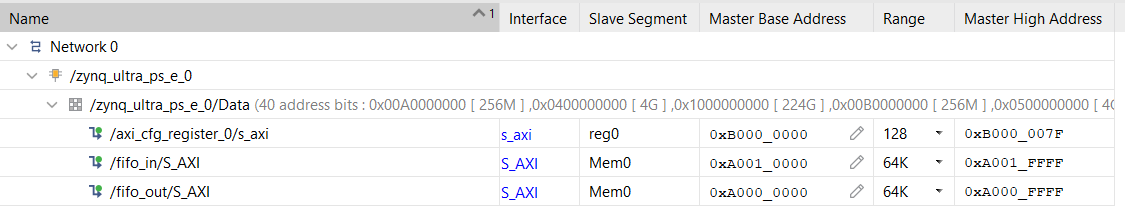
\includegraphics[width=1\textwidth]{images/addresses}
	\caption{Addresses definition.}
	\label{fig:addresses}
\end{figure}
The receive/transmit FIFO depth was set to 2048 byte. Regarding the other blocks, their configuration does not require any additional steps beyond what was covered in the previous chapters. Similarly, the generation of the bitstream and the .bin file follows the same process and does not require further explanation.



\section{Petalinux project}
The configuration of the PetaLinux project remains the same as explained in the previous chapter up to the rootfs configuration. However, when creating the driver, certain files need to be modified, requiring an update of the project. These modifications ensure the proper integration of the new software components.



\section{Driver implementation}
After successfully building the project, performing read/write operations on the memories and registers requires the definition of two additional components: a) the Driver, responsible for managing communication between the PS and the PL and b) the user program, which executes the operations using the driver to interact with the hardware. The driver must then be compiled into a .ko (Kernel Object) file, which can be loaded and executed on the KRIA board. The procedure to achieve this is quite complex, and even small mistakes can lead to errors. Therefore, careful attention is required at each step to ensure successful implementation.



The first step is to locate two files:
\begin{itemize}
	\item \textbf{system-user.dtsi} (found in \textit{project-spe/meta-user/recipes-bps/device-tree/files})
	
	\item \textbf{pl.dtsi} )
\end{itemize}
and open them with an editor. Down below is reported the code of pl.dtsi.
\vspace{0.1cm}
\begin{lstlisting}[language=C]
/dts-v1/;
/plugin/;
/ {
	fragment@0 {
		target = <&fpga_full>;
		overlay0: __overlay__ {
			#address-cells = <2>;
			#size-cells = <2>;
			firmware-name = "design_1_wrapper.bit.bin";
			resets = <&zynqmp_reset 116>;
		};
	};
	fragment@1 {
		target = <&amba>;
		overlay1: __overlay__ {
			afi0: afi0 {
				compatible = "xlnx,afi-fpga";
				config-afi = < 0 0>, <1 0>, <2 0>, <3 0>, <4 0>, <5 0>, <6 0>, <7 0>, <8 0>, <9 0>, <10 0>, <11 0>, <12 0>, <13 0>, <14 0xa00>, <15 0x000>;
			};
			clocking0: clocking0 {
				#clock-cells = <0>;
				assigned-clock-rates = <99999001>;
				assigned-clocks = <&zynqmp_clk 71>;
				clock-output-names = "fabric_clk";
				clocks = <&zynqmp_clk 71>;
				compatible = "xlnx,fclk";
			};
			clocking1: clocking1 {
				#clock-cells = <0>;
				assigned-clock-rates = <99999001>;
				assigned-clocks = <&zynqmp_clk 72>;
				clock-output-names = "fabric_clk";
				clocks = <&zynqmp_clk 72>;
				compatible = "xlnx,fclk";
			};
		};
	};
	fragment@2 {
		target = <&amba>;
		overlay2: __overlay__ {
			#address-cells = <2>;
			#size-cells = <2>;
			axi_cfg_register_0: axi_cfg_register@b0000000 {
				clock-names = "aclk";
				clocks = <&zynqmp_clk 71>;
				compatible = "xlnx,axi-cfg-register-1.0";
				reg = <0x0 0xb0000000 0x0 0x80>;
			};
			fifo_in: axi_fifo_mm_s@a0010000 {
				clock-names = "s_axi_aclk";
				clocks = <&zynqmp_clk 71>;
				compatible = "xlnx,axi-fifo-mm-s-4.3";
				reg = <0x0 0xa0010000 0x0 0x10000>;
				xlnx,axi-str-rxd-protocol = "XIL_AXI_STREAM_ETH_DATA";
				xlnx,axi-str-rxd-tdata-width = <0x20>;
				xlnx,axi-str-txc-protocol = "XIL_AXI_STREAM_ETH_CTRL";
				xlnx,axi-str-txc-tdata-width = <0x20>;
				xlnx,axi-str-txd-protocol = "XIL_AXI_STREAM_ETH_DATA";
				xlnx,axi-str-txd-tdata-width = <0x20>;
				xlnx,axis-tdest-width = <0x4>;
				xlnx,axis-tid-width = <0x4>;
				xlnx,axis-tuser-width = <0x4>;
				xlnx,data-interface-type = <0x0>;
				xlnx,has-axis-tdest = <0x0>;
				xlnx,has-axis-tid = <0x0>;
				xlnx,has-axis-tkeep = <0x0>;
				xlnx,has-axis-tstrb = <0x0>;
				xlnx,has-axis-tuser = <0x0>;
				xlnx,rx-cascade-height = <0x0>;
				xlnx,rx-enable-ecc = <0x0>;
				xlnx,rx-fifo-depth = <0x800>;
				xlnx,rx-fifo-pe-threshold = <0x5>;
				xlnx,rx-fifo-pf-threshold = <0x1fb>;
				xlnx,rx-has-ecc-err-inject = <0x0>;
				xlnx,s-axi-id-width = <0x4>;
				xlnx,s-axi4-data-width = <0x20>;
				xlnx,select-xpm = <0x0>;
				xlnx,tx-cascade-height = <0x0>;
				xlnx,tx-enable-ecc = <0x0>;
				xlnx,tx-fifo-depth = <0x200>;
				xlnx,tx-fifo-pe-threshold = <0x5>;
				xlnx,tx-fifo-pf-threshold = <0x1fb>;
				xlnx,tx-has-ecc-err-inject = <0x0>;
				xlnx,use-rx-cut-through = <0x0>;
				xlnx,use-rx-data = <0x1>;
				xlnx,use-tx-ctrl = <0x0>;
				xlnx,use-tx-cut-through = <0x0>;
				xlnx,use-tx-data = <0x0>;
			};
			fifo_out: axi_fifo_mm_s@a0000000 {
				clock-names = "s_axi_aclk";
				clocks = <&zynqmp_clk 71>;
				compatible = "xlnx,axi-fifo-mm-s-4.3";
				reg = <0x0 0xa0000000 0x0 0x10000>;
				xlnx,axi-str-rxd-protocol = "XIL_AXI_STREAM_ETH_DATA";
				xlnx,axi-str-rxd-tdata-width = <0x20>;
				xlnx,axi-str-txc-protocol = "XIL_AXI_STREAM_ETH_CTRL";
				xlnx,axi-str-txc-tdata-width = <0x20>;
				xlnx,axi-str-txd-protocol = "XIL_AXI_STREAM_ETH_DATA";
				xlnx,axi-str-txd-tdata-width = <0x20>;
				xlnx,axis-tdest-width = <0x4>;
				xlnx,axis-tid-width = <0x4>;
				xlnx,axis-tuser-width = <0x4>;
				xlnx,data-interface-type = <0x0>;
				xlnx,has-axis-tdest = <0x0>;
				xlnx,has-axis-tid = <0x0>;
				xlnx,has-axis-tkeep = <0x0>;
				xlnx,has-axis-tstrb = <0x0>;
				xlnx,has-axis-tuser = <0x0>;
				xlnx,rx-cascade-height = <0x0>;
				xlnx,rx-enable-ecc = <0x0>;
				xlnx,rx-fifo-depth = <0x200>;
				xlnx,rx-fifo-pe-threshold = <0x5>;
				xlnx,rx-fifo-pf-threshold = <0x1fb>;
				xlnx,rx-has-ecc-err-inject = <0x0>;
				xlnx,s-axi-id-width = <0x4>;
				xlnx,s-axi4-data-width = <0x20>;
				xlnx,select-xpm = <0x0>;
				xlnx,tx-cascade-height = <0x0>;
				xlnx,tx-enable-ecc = <0x0>;
				xlnx,tx-fifo-depth = <0x800>;
				xlnx,tx-fifo-pe-threshold = <0x5>;
				xlnx,tx-fifo-pf-threshold = <0x1fb>;
				xlnx,tx-has-ecc-err-inject = <0x0>;
				xlnx,use-rx-cut-through = <0x0>;
				xlnx,use-rx-data = <0x0>;
				xlnx,use-tx-ctrl = <0x1>;
				xlnx,use-tx-cut-through = <0x0>;
				xlnx,use-tx-data = <0x1>;
			};
		};
	};
};
\end{lstlisting}
\vspace{0.1cm}
Edit the system-user.dtsi file, which is initially empty, by creating the \textbf{amba\_pl} device tree node. Within this node: a) copy the afi node, b) include all components related to the memories instantiated in the Vivado design and c) copy the \textbf{clocking0} and \textbf{clocking1} components. The final system-user.dtsi file for this application is shown below.
\vspace{0.1cm}
\begin{lstlisting}[language=C]
/include/ "system-conf.dtsi"
/ {
	amba_pl: amba_pl {
		compatible = "simple-bus";
		ranges ;
		axi_cfg_register_0: axi_cfg_register@b0000000 {
			clock-names = "aclk";
			clocks = <&zynqmp_clk 71>;
			compatible = "xlnx,axi-cfg-register-1.0";
			reg = <0x0 0xb0000000 0x0 0x80>;
		};
		afi0: afi0 {
			compatible = "xlnx,afi-fpga";
			config-afi = < 0 0>, <1 0>, <2 0>, <3 0>, <4 0>, <5 0>, <6 0>, <7 0>, <8 0>, <9 0>, <10 0>, <11 0>, <12 0>, <13 0>, <14 0xa00>, <15 0x000>;
		};
		clocking0: clocking0 {
			#clock-cells = <0>;
			assigned-clock-rates = <99999001>;
			assigned-clocks = <&zynqmp_clk 71>;
			clock-output-names = "fabric_clk";
			clocks = <&zynqmp_clk 71>;
			compatible = "xlnx,fclk";
		};
		clocking1: clocking1 {
			#clock-cells = <0>;
			assigned-clock-rates = <99999001>;
			assigned-clocks = <&zynqmp_clk 72>;
			clock-output-names = "fabric_clk";
			clocks = <&zynqmp_clk 72>;
			compatible = "xlnx,fclk";
		};
		fifo_in: axi_fifo_mm_s@a0010000 {
			clock-names = "s_axi_aclk";
			clocks = <&zynqmp_clk 71>;
			compatible = "xlnx,axi-fifo-mm-s-4.3";
			reg = <0x0 0xa0010000 0x0 0x10000>;
			xlnx,axi-str-rxd-protocol = "XIL_AXI_STREAM_ETH_DATA";
			xlnx,axi-str-rxd-tdata-width = <0x20>;
			xlnx,axi-str-txc-protocol = "XIL_AXI_STREAM_ETH_CTRL";
			xlnx,axi-str-txc-tdata-width = <0x20>;
			xlnx,axi-str-txd-protocol = "XIL_AXI_STREAM_ETH_DATA";
			xlnx,axi-str-txd-tdata-width = <0x20>;
			xlnx,axis-tdest-width = <0x4>;
			xlnx,axis-tid-width = <0x4>;
			xlnx,axis-tuser-width = <0x4>;
			xlnx,data-interface-type = <0x0>;
			xlnx,has-axis-tdest = <0x0>;
			xlnx,has-axis-tid = <0x0>;
			xlnx,has-axis-tkeep = <0x0>;
			xlnx,has-axis-tstrb = <0x0>;
			xlnx,has-axis-tuser = <0x0>;
			xlnx,rx-cascade-height = <0x0>;
			xlnx,rx-enable-ecc = <0x0>;
			xlnx,rx-fifo-depth = <0x800>;
			xlnx,rx-fifo-pe-threshold = <0x5>;
			xlnx,rx-fifo-pf-threshold = <0x1fb>;
			xlnx,rx-has-ecc-err-inject = <0x0>;
			xlnx,s-axi-id-width = <0x4>;
			xlnx,s-axi4-data-width = <0x20>;
			xlnx,select-xpm = <0x0>;
			xlnx,tx-cascade-height = <0x0>;
			xlnx,tx-enable-ecc = <0x0>;
			xlnx,tx-fifo-depth = <0x200>;
			xlnx,tx-fifo-pe-threshold = <0x5>;
			xlnx,tx-fifo-pf-threshold = <0x1fb>;
			xlnx,tx-has-ecc-err-inject = <0x0>;
			xlnx,use-rx-cut-through = <0x0>;
			xlnx,use-rx-data = <0x1>;
			xlnx,use-tx-ctrl = <0x0>;
			xlnx,use-tx-cut-through = <0x0>;
			xlnx,use-tx-data = <0x0>;
		};
		fifo_out: axi_fifo_mm_s@a0000000 {
			clock-names = "s_axi_aclk";
			clocks = <&zynqmp_clk 71>;
			compatible = "xlnx,axi-fifo-mm-s-4.3";
			reg = <0x0 0xa0000000 0x0 0x10000>;
			xlnx,axi-str-rxd-protocol = "XIL_AXI_STREAM_ETH_DATA";
			xlnx,axi-str-rxd-tdata-width = <0x20>;
			xlnx,axi-str-txc-protocol = "XIL_AXI_STREAM_ETH_CTRL";
			xlnx,axi-str-txc-tdata-width = <0x20>;
			xlnx,axi-str-txd-protocol = "XIL_AXI_STREAM_ETH_DATA";
			xlnx,axi-str-txd-tdata-width = <0x20>;
			xlnx,axis-tdest-width = <0x4>;
			xlnx,axis-tid-width = <0x4>;
			xlnx,axis-tuser-width = <0x4>;
			xlnx,data-interface-type = <0x0>;
			xlnx,has-axis-tdest = <0x0>;
			xlnx,has-axis-tid = <0x0>;
			xlnx,has-axis-tkeep = <0x0>;
			xlnx,has-axis-tstrb = <0x0>;
			xlnx,has-axis-tuser = <0x0>;
			xlnx,rx-cascade-height = <0x0>;
			xlnx,rx-enable-ecc = <0x0>;
			xlnx,rx-fifo-depth = <0x200>;
			xlnx,rx-fifo-pe-threshold = <0x5>;
			xlnx,rx-fifo-pf-threshold = <0x1fb>;
			xlnx,rx-has-ecc-err-inject = <0x0>;
			xlnx,s-axi-id-width = <0x4>;
			xlnx,s-axi4-data-width = <0x20>;
			xlnx,select-xpm = <0x0>;
			xlnx,tx-cascade-height = <0x0>;
			xlnx,tx-enable-ecc = <0x0>;
			xlnx,tx-fifo-depth = <0x800>;
			xlnx,tx-fifo-pe-threshold = <0x5>;
			xlnx,tx-fifo-pf-threshold = <0x1fb>;
			xlnx,tx-has-ecc-err-inject = <0x0>;
			xlnx,use-rx-cut-through = <0x0>;
			xlnx,use-rx-data = <0x0>;
			xlnx,use-tx-ctrl = <0x1>;
			xlnx,use-tx-cut-through = <0x0>;
			xlnx,use-tx-data = <0x1>;
		};
	};
};
\end{lstlisting}
\vspace{0.1cm}
After this procedure it is necessary to rebuild the project. Once the building is complete, it is possible to generate the .wic image and proceed with SDC card flashing.

Now, the driver can be generated and compiled. An automatic Python-based generator is used to create the driver, which takes as input: a) the name of the driver b) the path to system-user.dtsi and c) the name of an input FIFO. The generator produces the driver's template files (.c and .h). The required steps are the following:
\begin{enumerate}
	\item Create the driver module using the command
	\vspace{0.1cm}
	\begin{lstlisting}[language=bash]
		petalinux-create -t modules --name driver_name --enable	\end{lstlisting}
	
	\item Copy the template files into \textit{project-spec/meta-user/recipes-modules/driver\_name/files/}.
	
	\item Modify the Makefile to include the path to the .h file in the \textbf{MY\_CFLAGS} line. Not including the path will result in an error, as PetaLinux will be unable to locate such file. The updated Makefile is shown below:
	\vspace{0.1cm}
	\begin{lstlisting}[language=make]
		obj-m := blinkdriver.o
		
		MY_CFLAGS += -g -DDEBUG -I /data/devel/kria_mb/ptlnx/prj/blink_mk_VIII/project-spec/meta-user/recipes-modules/blinkdriver/files
		ccflags-y += ${MY_CFLAGS}
		
		SRC := $(shell pwd)
		
		all:
		$(MAKE) -C $(KERNEL_SRC) M=$(SRC)
		
		modules_install:
		$(MAKE) -C $(KERNEL_SRC) M=$(SRC) modules_install
		
		clean:
		rm -f *.o *~ core .depend .*.cmd *.ko *.mod.c
		rm -f Module.markers Module.symvers modules.order
		rm -rf .tmp_versions Modules.symvers
	\end{lstlisting}

	\item Build the driver using:Build the driver using
	\vspace{0.1cm}
	\begin{lstlisting}[language=bash]
		petalinux-build -c driver_name	\end{lstlisting}
	
	\item Locate the .ko file and copy it, through ssh, to the KRIA along with the .h file. Move also the .bin file.
	
	\item Applying the same procedure described above program the FPGA.
	
	\item With the command 
	\vspace{0.1cm}
	\begin{lstlisting}[language=bash]
		sudo insmod driver_name.ko	\end{lstlisting}
	launch the driver in the KRIA. 
	
	\item This last step has to be done after the program that will make use of the driver has been written and complied. Once the program is done then type
	\vspace{0.1cm}
	\begin{lstlisting}[language=bash]
		./program_name	\end{lstlisting}
	and now everything should be working properly.
\end{enumerate}




\section{Test code}
The test code is divided into three main sections:
\begin{itemize}
	\item \textbf{System initialization} In this section, all necessary variables are initialized along with the driver (blinkdriver). If an error occurs during driver initialization for any reason, the variable fd will take a negative value (likely -1), causing the system to throw an error. If the driver initializes correctly, both memory blocks are cleared. Finally, the read/write functionality of the cfg\_register is tested.
	
	\item \textbf{Memory writing} In the second section a series of values are written in the FIFO IN memory via the FIFO OUT memory. To verify then the effective success of the operation, the FIFO IN memory length is displayed. 
	
	\item \textbf{Memory reading} In the last section, the values written into the FIFO IN memory are read and displayed in the terminal window.
\end{itemize}
\vspace{0.1cm}
\begin{lstlisting}[language=C]
#include <sys/ioctl.h>
#include <fcntl.h>
#include <stdlib.h>
#include <string.h>
#include <errno.h>
#include <unistd.h>
#include <stdio.h>
#include "blinkdriver.h"

int main(int argc, char *argv[])
{
	\\ Initialization ----------------------------------------------
	int i, fd, reg, len, val;
	fd = open("/dev/blinkdriver", O_RDWR);
	if(fd < 0)
	{
		printf("Error\n");
		exit(0);
	}
	ioctl(fd, BLINKDRIVER_CLEAR_FIFO_IN, 0);
	ioctl(fd, BLINKDRIVER_CLEAR_FIFO_OUT, 0);
	
	reg = 0;
	ioctl(fd, BLINKDRIVER_SET_AXI_CFG_REGISTER_0, &reg);
	usleep(100);
	reg = 123;
	ioctl(fd, BLINKDRIVER_SET_AXI_CFG_REGISTER_0, &reg);
	reg = 0;
	ioctl(fd, BLINKDRIVER_GET_AXI_CFG_REGISTER_0, &reg);
	printf("Reg: %d\n", reg);
	usleep(100);
	
	\\ Memory writing ----------------------------------------------
	for(i = 0; i < 10; i++)
	{
		val = i * 10;
		ioctl(fd, BLINKDRIVER_SET_FIFO_OUT_VAL, &val);
		ioctl(fd, BLINKDRIVER_GET_FIFO_OUT_LEN, &len);
		printf("Out Vacancy: %d\n", len);
	}
	usleep(100);
	ioctl(fd, BLINKDRIVER_GET_FIFO_IN_LEN, &len);
	printf("FIFO Len: %d\n", len);
	
	\\ Memory reading ----------------------------------------------
	ioctl(fd, BLINKDRIVER_START_READ, 0);
	for(i = 0; i < len; i++)
	{
		read(fd, &val, 4);
		printf("FIFO Val: %d\n", val);
	}

	ioctl(fd, BLINKDRIVER_GET_FIFO_IN_LEN, &len);
	printf("FIFO Len: %d\n", len);
	ioctl(fd, BLINKDRIVER_START_READ, 0);
	
	return 0;
}
\end{lstlisting}
\vspace{0.1cm}
The code reported shows a simple, yet effective way to demonstrate how to perform R/W operations. Once the code is completed it has to be copied into the same folder as the diver's .h file. To compile it use the command
\vspace{0.1cm}
\begin{lstlisting}[language=bash]
	gcc code_name.c -o code_name	\end{lstlisting}
\vspace{0.1cm}
and then follow the procedure described in point 8 above.